\subsubsection{Functional Requirements}
\begin{itemize}
  \item The system must unlock the right car when an user requests to.
  \item The system must not unlock any car that does not match the user's reservation and the submitted vehicle-PIN.
  \item The system must switch the car state to "IN USE" only when the user unlocks it.
  \item The system must set the car state to "FREE" only when the user leaves it.
  \item The system must close the reservation as soon as the car state is set to "IN USE".
  \item The onboard computer must unlock the car commands if and only if the right PIN code has been inserted.
  \item The system must calculate the current charges and display it through the onboard computer.
  \item The system must correctly detect accidents and set the car state to "OUT OF SERVICE".
  \item The system must correctly detect when a car is outside the safe-area and prevent the user from ending the ride.
  \item If a car is left at more than 3Km from the nearest power grid station or with more than 80\% of the battery empty, its state must be set to "OUT OF SERVICE" and an operator must charge it on-site and notify the system to set its state to "FREE" again.
\end{itemize}


\subsubsection{Scenario 1}
Anna has a pending reservation and is just in front of her PowerEnJoy car, she requests to unlock the car through the application end enters. She is then asked for her PIN code and after a correctness check the engine is unlocked and Anna starts driving. When at destination, she notices that the car is not parked inside the safe-area so she moves it until inside and leaves the car after parking it, immediately receiving a payment notification.


\subsubsection{Scenario 2}
Michael and his two brothers are far from home and its really late, the subway is already closed and since they have seen a PowerEnJoy vehicle near them, they decided to reserve it and proceed with the unlock procedure. After entering his PIN, Michael starts driving and once at home they park and leave the car. But the system notices that the battery level is below 20\% and (even if two additional passengers were taken) Michael is charged 30\% more.


\subsubsection{Mockups}
\begin{figure}[!ht]
  \centering
  \vspace{0.2cm}
  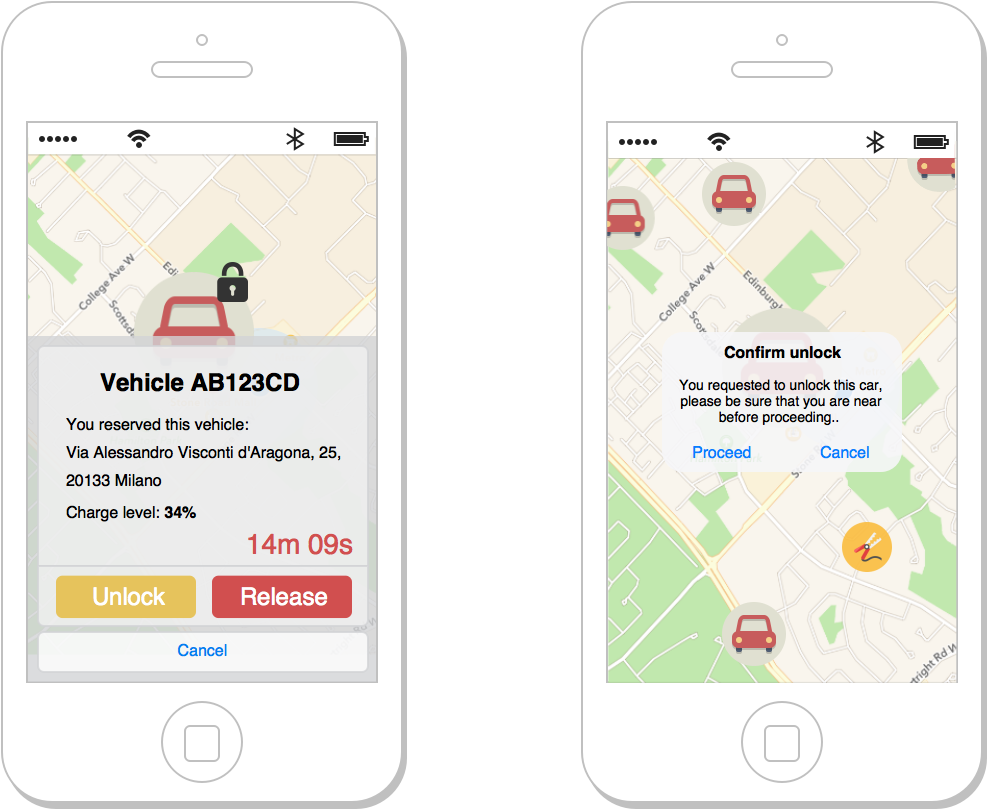
\includegraphics[width=0.75\textwidth]{/RASD/System_Functions/use_car_mockup}\\
  \vspace{0.2cm}
  %\caption{Mockup for the use-car use case} 
  \label{fig:use_car_mockup} 
\end{figure}
% maybe home page mockup here 


\subsubsection{Use-case table}
\begin{center}
  \begin{tabular}{ l | p{10cm} }
    \hline
    Actors & User\\ \hline
    Goal & G\ref{itm:goal-registration}\\ \hline
    Entry conditions & The Guest is near the car with a matching valid reservation active. 
     \\ \hline
    Flow of events &
    \begin{itemize} % todo: shrink items
      \item The User requests to unlock the car through the application, the unlock request must include the vehicle-PIN.
      \item The system checks the validity of the request and unlocks the car, setting its state to "IN USE".
      \item The User enters the car and digits the PIN on the onboard computer.
      \item The PIN is checked and the engine is unlocked.
      \item The User uses the car and is showed the charges in real-time.
      \item The User parks in a safe area and leaves the car in order to end the rental.
      \item The system charges the user and tags the car as "FREE".
    \end{itemize} \\ \hline
    Exit conditions & The User has left the car and has no active reservations, he has been charged for the rental. The car state is "FREE". \\ \hline
  	Exceptions & 
    \begin{itemize}
      \item The reservation expires just before the unlock request (the system notifies an InvalidReservation exception).
      \item An accident/engine fault occurs (the system tags the car as "OUT OF SERVICE" and requests maintenance).
      \item The user doesn't leave the car in a safe area (the system tags the car as "OUT OF SERVICE").
    \end{itemize} \\ \hline
  \end{tabular}
\end{center}

\newpage
\subsubsection{Sequence diagram}
\begin{figure}[!ht]
  \centering
  \vspace{0.2cm}
  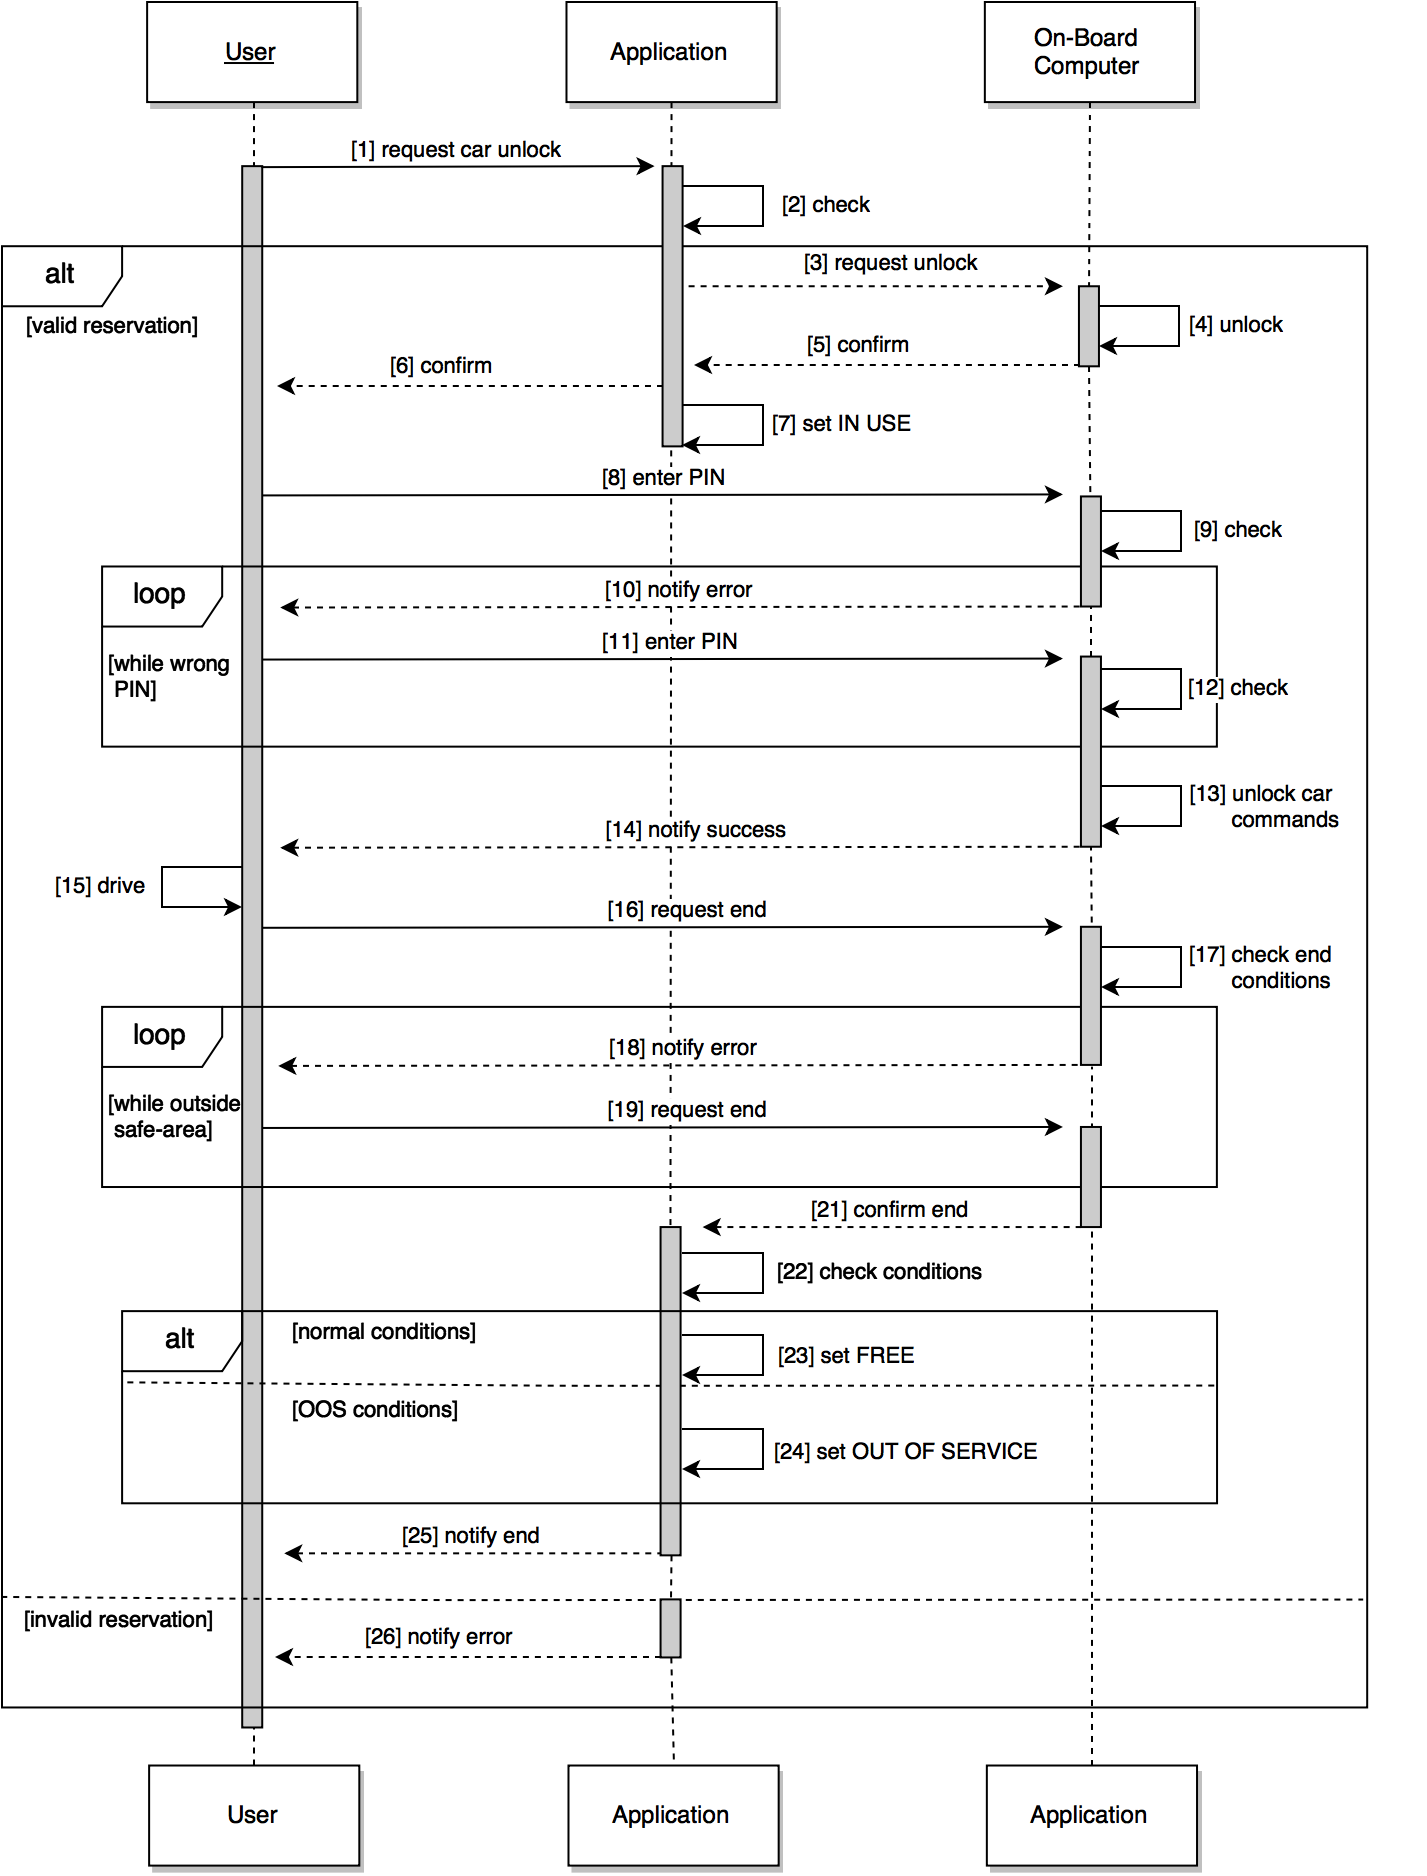
\includegraphics[width=0.7\textwidth]{/RASD/System_Functions/use_car_sequence}\\
  \vspace{0.4cm}
  %\caption{Sequence diagram for the use-car procedure} 
  \label{fig:use_car_sequence} 
\end{figure}

\subsubsection{State machine diagram}
\begin{figure}[!ht]
  \centering
  \vspace{0.2cm}
  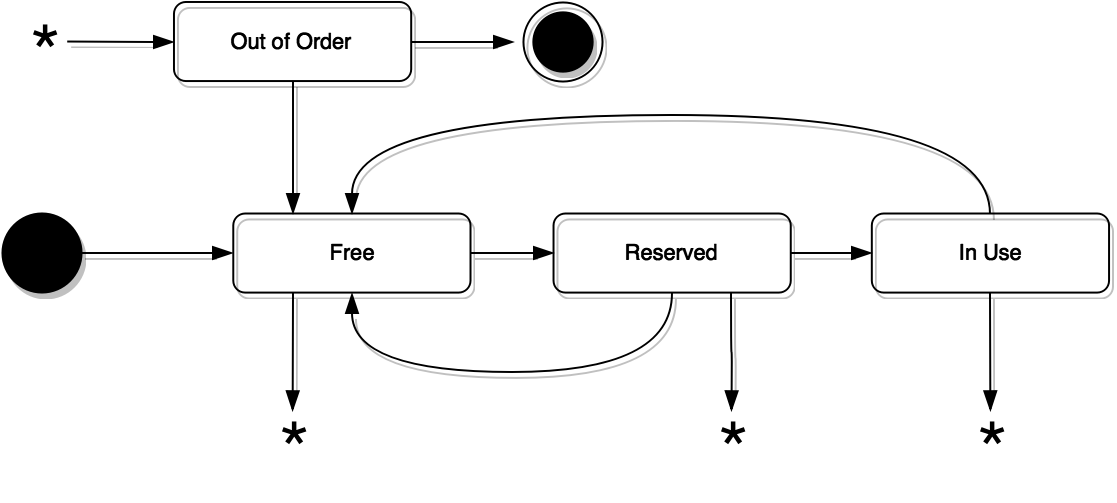
\includegraphics[width=0.6\textwidth]{/RASD/System_Functions/car_state_chart}\\
  \vspace{0.4cm}
  %\caption{Diagram representing all the possible car states} 
  \label{fig:car_state_chart} 
\end{figure}
